\xchapter{Estudo Experimental}{}
\label{estudo-experimental}

Este capítulo apresenta o processo de avaliação utilizado para medir a precisão do
sistema de identificação de momentos oportunos e inoportunos proposto. As seções deste
capítulo estão organizadas da seguinte forma: A seção x lorem ipsum.

\section{Metodologia}
\label{metodologia}

O desempenho da proposta foi avaliado a partir de um experimento executado durante
situações reais de direção em um percurso em algumas ruas da cidade de Salvador -
Bahia. O percurso está apresentado na figura \ref{percurso}.

\begin{figure}[h]
\centering
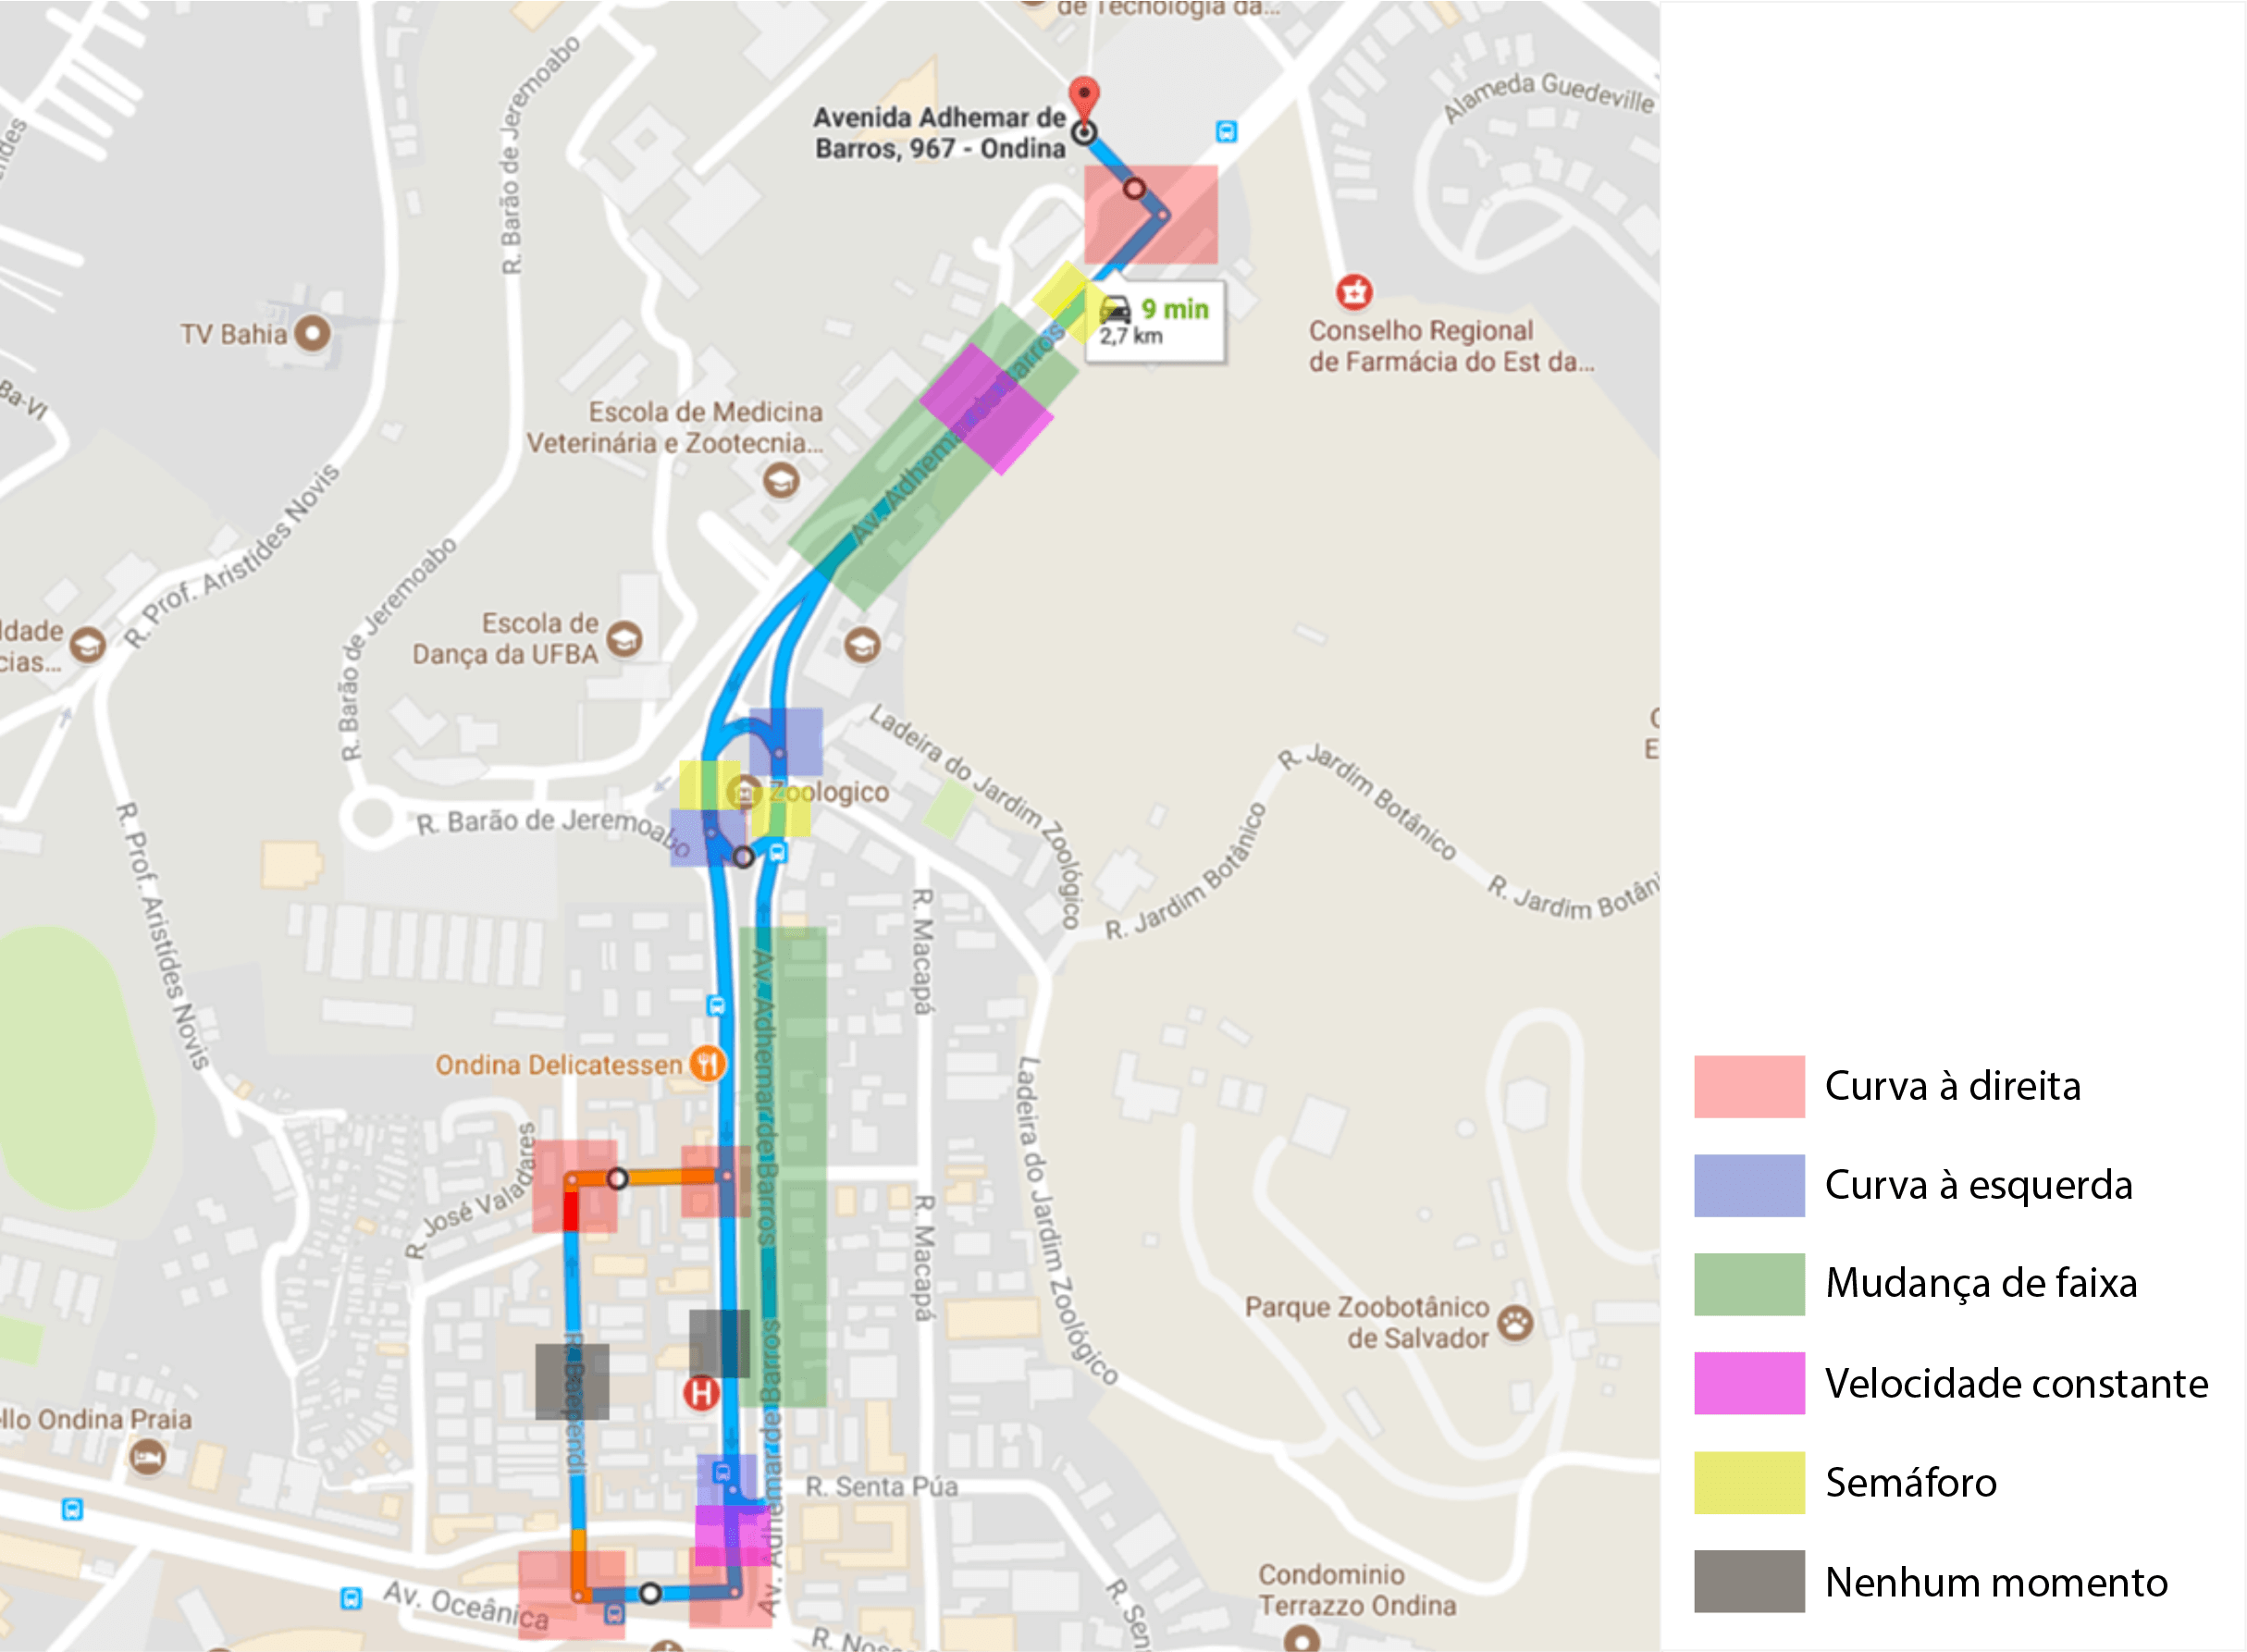
\includegraphics[width=0.53\textwidth]{images/percurso.png}
\caption{Percurso realizado no experimento de avaliação}
\label{percurso}
\end{figure}

O trajeto é composto de 5 curvas à direita, 3 curvas à esquerda e 2 lugares com mudança de faixa.
O experimento foi realizado com 3 voluntários, todos dirigindo em seu próprio carro.

O smartphone escolhido para realizar o experimento foi um OnePlus One com as seguintes características
\cite{oneplusone}:

\begin{enumerate}
  \item Sistema Operacional: Cyanogen OS 13.1.2 (Android Marshmallow 6.0.1)
\end{enumerate}
